\documentclass[12pt,a4paper,oneside]{report}

\usepackage{enumitem}
\usepackage{setspace}
\usepackage[none]{hyphenat}
\usepackage{algorithm} 
\usepackage{algorithmic}
\usepackage{amsmath}
\usepackage{amsfonts}
\usepackage{graphicx}
\usepackage{caption}
\usepackage{subcaption}
\graphicspath{ {image/} }

\newcommand{\INDSTATE}[1][1]{\STATE\hspace{#1\algorithmicindent}}

\begin{document}

%===============================================================================
% Start of Cover Page
%===============================================================================
\title{\Huge\textbf{The iPad Crusher \vfill
	\large Project Report \\ \bigskip
	for \\ \bigskip
	CS2309 CS Research Methodology \\ \bigskip
	\large AY15/16 Sem 1 \vfill}
	}
\author{
	Department of Computer Science \\\\
	School of Computing \\\\
	National University of Singapore}
%\date{}

\maketitle
%===============================================================================
% End of Cover Page
%===============================================================================

\pagenumbering{roman}

%===============================================================================
% Start of Title Page
%===============================================================================
\begin{titlepage}
\addcontentsline{toc}{chapter}{Title Page}
\thispagestyle{plain}
\begin{center}
\textbf{\Huge The iPad Crusher \vfill
	\large Project Report \\ \bigskip
	for \\ \bigskip
	CS2309 CS Research Methodology \\ \bigskip
	AY15/16 Sem 1} \vfill \vfill
\large Members: \\ \bigskip
\begin{minipage}[t]{0.3\textwidth}
\begin{flushleft}
Lai Hoang Dung \\ \bigskip
Lim Kiat \\ \bigskip
Liu Xinan \\ \bigskip
Tran Tien Dat
\end{flushleft}
\end{minipage}
\begin{minipage}[t]{0.3\textwidth}
\begin{flushright}
A0131125Y \\ \bigskip
A0124099B \\ \bigskip
A0130195M \\ \bigskip
A0131140E
\end{flushright}
\end{minipage} \vfill
Supervisor: \\ \bigskip
Prof. Sim Khe Chai
\end{center}
\end{titlepage}
%===============================================================================
% End of Title Page
%===============================================================================

%===============================================================================
% Start of Abstract
%===============================================================================
\begin{abstract}
\setcounter{page}{2}
\thispagestyle{plain}
\onehalfspacing
\addcontentsline{toc}{chapter}{Abstract}
In this project, we were asked to design the game logic for ``iPad Crusher'', an iOS game that Prof. Sim is developing as an adaptation to the Egg Dropping Problem. Given a certain number of iPads and strength levels, the player is asked to find the lowest strength level that would break an iPad. Similar to the Egg Dropping Puzzle, the goal of the game is to find the best strategy so that it involves the fewest number of crushing in the worst-case scenario. \\\\
In this report we present two approaches in designing the game logic, the first is the original solution that we came up with, which is to generate the cost table and make the game decisions based on the costs. The second approach is one that Prof. Sim briefly mentioned, which decides based on the optimum level stored in a table. We would discuss the advantages and disadvantages of each of the two approaches, as well as different implementations of them. Lastly we would discuss some interesting extension of the problem such as adding an extra cost for breaking an iPad, and a variant of it with unlimited number of iPads, etc. In the end we conclude that for the original game logic, the cost table approach would be the better choice, whereas for some extensions, the decision tree approach would be better.

\subsubsection*{Subject Descriptors:\\}
\begin{description}[labelindent=1cm]
	\item[I.2.8] Dynamic Programming
	\item[K.8.0] Games
	\item[G.2.1] Combinatorics
\end{description}

\subsubsection{Keywords:}
\begin{description}[labelindent=1cm]
	\item Game Logic, Egg Dropping, Dynamic Programming, Combinatorics
\end{description}

\end{abstract}
%===============================================================================
% End of Abstract
%===============================================================================

%===============================================================================
% Start of Acknowledgements
%===============================================================================
\renewcommand{\abstractname}{Acknowledgements}
\begin{abstract}
\setcounter{page}{3}
\thispagestyle{plain}
\onehalfspacing
\addcontentsline{toc}{chapter}{Acknowledgements}
We could like to thank Prof. Sim Khe Chai for the patience and guidance along the semester. Without Prof. Sim, we would not have gone this far. We would also like to thank our fellow classmates for the interesting discussions we had in our tutorial regarding this project that made us think deeper about the problem.
\end{abstract}
%===============================================================================
% End of Acknowledgements
%===============================================================================

\onehalfspacing
\tableofcontents
\thispagestyle{empty}
\addtocontents{toc}{\protect\thispagestyle{empty}}
\pagenumbering{arabic}

%===============================================================================
% Start of Chapter 1
%===============================================================================
\chapter{Introduction}
\setcounter{page}{1}
The egg dropping puzzle is a well known one and an example most often used to illustrate dynamic programming as a concept in computer science. As an adaptation to the egg dropping puzzle, we were tasked to design the game logic for ``iPad Crusher'', an iOS game that our Prof. is developing. The problem involves $N$ number of iPads available and $L$ strength levels the player can use to crush the iPads. The goal of the game is to find the best strategy so that it involves the fewest number of crushing in the worst-case scenario. In the process leading up to the actual formulation of the game logic, we were guided to first come up with a brute-force approach to finding the best strategy. Thereafter, since the egg dropping puzzle can be solved using dynamic programming, we have done the same for our problem. With the dynamic programming solution, we were then able to design the game logic, which determines whether the iPad should survive, given the strength level that the user specifies. The game logic is one where it always simulates the worst-case scenario. This means that when a player chooses a strength level he/she wishes to use, the game logic will decide whether to crush the iPad depending on the choice that will result in more tries needed using a best strategy. As a further extension, we explored the case where we have to factor in a fixed iPad cost for each crushing of an iPad, as well as when the iPad cost changes as different numbers of iPads get crushed.

%===============================================================================
% End of Chapter 1
%===============================================================================

%===============================================================================
% Start of Chapter 2
%===============================================================================
\chapter{Existing work}
I put random chapter titles here. Feel free to change. And this is how you cite a source \cite{randomblogpost}.

\section{What does the fox say?}
\subsection{Introduction}
Lorem ipsum dolor sit amet, consectetur adipiscing elit. Duis quis lacus posuere, tincidunt mauris vitae, bibendum sapien. Suspendisse a eros pretium, pretium libero eget, ornare ante. Donec efficitur gravida pellentesque. Curabitur sit amet pulvinar tortor. In eu risus commodo, elementum tellus ac, commodo mauris. Vestibulum ante ipsum primis in faucibus orci luctus et ultrices posuere cubilia Curae; Integer hendrerit arcu sem, convallis dignissim nisi faucibus at. Praesent ut rutrum libero, sollicitudin blandit dui. Donec mi nisi, cursus quis accumsan et, molestie ut nisi. Sed egestas enim in dolor tincidunt dictum. Sed eu semper sem. Sed elementum augue ac pretium eleifend. Ut massa tortor, rhoncus a mi ac, congue ullamcorper eros. Maecenas imperdiet orci quis dui rhoncus, id rhoncus mi condimentum. Nunc blandit egestas leo, sit amet porttitor mi malesuada nec. Pellentesque id bibendum purus, a porta risus. \\\\

%===============================================================================
% End of Chapter 2
%===============================================================================

%===============================================================================
% Start of Chapter 3
%===============================================================================
\chapter{The cost table approach}
The first approach that came into our mind was to pre-compute an $N \times L$ two dimensional table containing the number of crushing needed for $N$ number of iPads and $L$ strength levels in the worst-case scenario. When the user choose a certain strength level, we will look up the costs for the upper sub-problem and the lower sub-problem in the table, compare them to decide whether the iPad should break at that strength level or not.

\section{Detailed description}
Let us define the cost of a game state $(N, L)$ to be the minimum number of crushing using $N$ number of iPads and for $L$ strength levels. \\\\
In a game level with $N$ number of iPads and $L$ strength levels, the user chooses to crush at strength level $x$:
\begin{itemize}
\item if the iPad breaks, the game state becomes $N - 1$ number of iPads and $x - 1$ strength levels.
\item if the iPad does not break, the game state becomes $N$ number of iPads and $L - x$ strength levels.
\end{itemize}
We can compute the cost of $(N, L)$ by recursively compute all possible sub-problems, the cost of $(N, L)$ would be $(1 + \text{cost of the minimum-cost sub-problem})$. Here are some base cases:
\begin{itemize}
\item if $N = 1$, the cost would be $L$ because the only way to find the correct strength is to try one by one from the lowest strength level to the highest strength level. In the worst-case, the iPad only breaks at the highest strength level, so it will need $L$ number of crushing.
\item if $L = 1$, the cost will be 1 since there is only one strength level to be crushed at.
\end{itemize}
Let $C(N, L)$ denote the cost for $N$ iPads and $L$ strength levels. \\
The recurrence is
\[
C(N, L) = 
\begin{cases}
L & \text{if $N = 1$} \\
1 & \text{if $L = 1$} \\
1 + min_{x \in [1, L]}(max(C(N - 1, x - 1), C(N, L - x))) & \text{otherwise}
\end{cases}
\]
So all we need is to compute a $N \times L$ two dimensional table for each possible combination of $N$ and $L$. For the game logic, if the user chooses to crush at strength level $x$, we will look up 
\begin{itemize}
\item $C(N - 1, x - 1)$ (cost of the remaining sub-problem if the iPad breaks)
\item $C(N, L - x)$ (cost of the remaining sub-problem if the iPad does not break)
\end{itemize}
in the cost table, if $C(N - 1, x - 1) > C(N, L - x)$, i.e. it will require more cost if the iPad breaks, then we will break the iPad. If $C(N - 1, x - 1) < C(N, L - x)$, i.e. it requires more cost if the iPad does not break, then we will not break the iPad. For cases when $C(N - 1, x - 1) = C(N, L - x)$, we can randomize the decision so that the game path will not always be the same.

\section{A brute force algorithm}
A naive way to implement this approach would be to compute every cell in the $N \times L$ cost table individually using the following algorithm:
\begin{algorithm}
\caption{$C(N, L)$}
\begin{algorithmic}[1]
\IF{$N = 1$}
	\RETURN $L$
\ELSIF{$L = 1$}
	\RETURN $1$
\ENDIF
\STATE $best \leftarrow \infty$
\FORALL{$x \in [1, L]$}
	\STATE $result = max(C(N - 1, x - 1), C(N, L - x))$
	\IF{$result < best$}
		\STATE $best \leftarrow result$
	\ENDIF
\ENDFOR
\RETURN $best + 1$
\end{algorithmic}
\end{algorithm}
~\\
Clearly this algorithm runs in exponential time. In fact, computing the cost for a game state $(N, L)$ involves the computation of game states with lower $N$ or lower $L$. Therefore there is a lot of repeated computation here. In the next section we will talk about how to avoid such redundant computations.

\section{A dynamic programming algorithm}
Based on the naive brute-force algorithm, we have derived a dynamic programming algorithm which avoids the unnecessary repeated computations and makes computing the cost for large problems more practical. \\\\
As we mentioned in the last section, using the brute-force algorithm, the computation of a larger problem involves computing a number of smaller problems, therefore it exhibits the optimal substructure property. Moreover, different problems might need to compute the same sub-problems, therefore it exhibits the overlapping sub-problem property. Hence, we can speed up the computation of it by using dynamic programming. \\\\
Instead of computing each cell individually and fill in the table, we initialize all the base cases and then fill in the table row by row and make use the already computed values to compute the new values. Here's the pseudo-code:
\begin{algorithm}
\caption{$makeTable(N, L)$}
\begin{algorithmic}[1]
\STATE $table \leftarrow 2DTable(N, L)$
\FOR{$i = 1$ \TO $N$}
	\STATE $table[i][1] = 1$
\ENDFOR
\FOR{$i = 1$ \TO $L$}
	\STATE $table[1][i] = i$
\ENDFOR
\FOR{$i = 1$ \TO $N$}
	\FOR{$j = 1$ \TO $L$}
		\STATE $best \leftarrow \infty$
		\FOR{$k = 1$ \TO $j$}
			\STATE $result = max(table(i - 1, k - 1), table(i, j - x))$
			\IF{$result < best$}
				\STATE $best \leftarrow result$
			\ENDIF
		\ENDFOR
		\STATE $table[i][j] = best + 1$
	\ENDFOR
\ENDFOR
\end{algorithmic}
\end{algorithm}
~\\
Using the dynamic programming algorithm, we can reduce the running time of the algorithm to $O(NL^2)$. This is because for each of the $N \times L$ entries, we only need at most $L$ comparisons to get the result. \\\\
It is capable of computing the cost with hundreds of strength levels and tens of iPads, whereas the brute-force algorithm is only capable of computing problems with around 20 strength levels and several iPads.
\section{Pros and Cons}

%===============================================================================
% End of Chapter 3
%===============================================================================

%===============================================================================
% Start of Chapter 4
%===============================================================================
\chapter{The optimum level approach}
Through the course of doing the project, Prof. Sim briefly mentioned about an approach that came naturally to him but was different from the cost table approach that every team in the class came up with. His approach was basically storing the optimum strength level to use in each cell of a $N$ by $L$ table. The optimum strength level is defined as the level of strength that the player should use such that he will require the least number of turns to solve the game in the worst case scenario. When we need to decide if an iPad should be crushed given a strength level input, we look up the table and compare the given level input against the optimum input to make the decision. As this approach seemed different from our original approach, we have decided to look more into it to see if it is a viable solution, along with its advantages and disadvantages.

\section{Description of approach}
The idea behind the approach is simple. By knowing the optimum strength level to use at each stage of the game, we can simply decide whether to crush the iPad or not. If the player inputs a strength level that is lower than the optimum strength level, the iPad will not be crushed. If the input strength level is higher than the optimum level, the iPad will be crushed.

\section{Viability of approach}
Following an extensive discussion we had about this particular approach, we came to realise that the approach will only give us the worst case scenario if it satisfies two conditions. Firstly, given a game state of $N$ iPads and $L$ strength levels $G(N,L)$, there can be a number of different levels that are all optimal. Amongst these optimal strength levels, the largest level should be chosen as the optimum level. The second condition is that if the player decides to use the optimum strength level, then the game logic should make the decision to crush the iPad.

Let us explore the reasoning behind these two conditions using Figure 4.1 on the following page. Figure 4.1 shows us two optimal decision trees, each of height 7, that can be used to solve the game state $G(2,30)$. The number in each node represents the strength level to use as a best strategy. If the iPad gets crushed, we will move down to the right subtree, and if the iPad is not crushed, then we move down the left subtree. With a height of 7, it means that at the very least, a player must make 8 attempts in order to win the game, and any situation that results in less will be because of a wrong decision made by the game logic.

The difference between these two trees is that tree (a) has 2 as its root node while tree (b) has 8, which is the optimum level that corresponds to the trees. The strength levels 2 and 8 are also the smallest and largest values of all the possible values that give an optimal decision tree of height 7. 

With these two examples, imagine that we take 2 as the optimum level. In the event that the player wants to use a strength level of 3 to crush the iPad, the game logic will decide to crush the iPad, leaving the player with 1 iPad left and only 2 more levels to test. This means that the game can be solved using 3 attempts (continue testing level 1 and level 2 using the last iPad), which is not the worst case scenario. However, if we take 8 as the optimum level, when the player uses a strength of level 3, the game logic will decide not to crush the iPad, which is the correct decision to make as it results in a worse scenario compared to the decision to crush the iPad. 

\begin{figure}[H]
	\centering
	\begin{subfigure}{0.68\textwidth}
		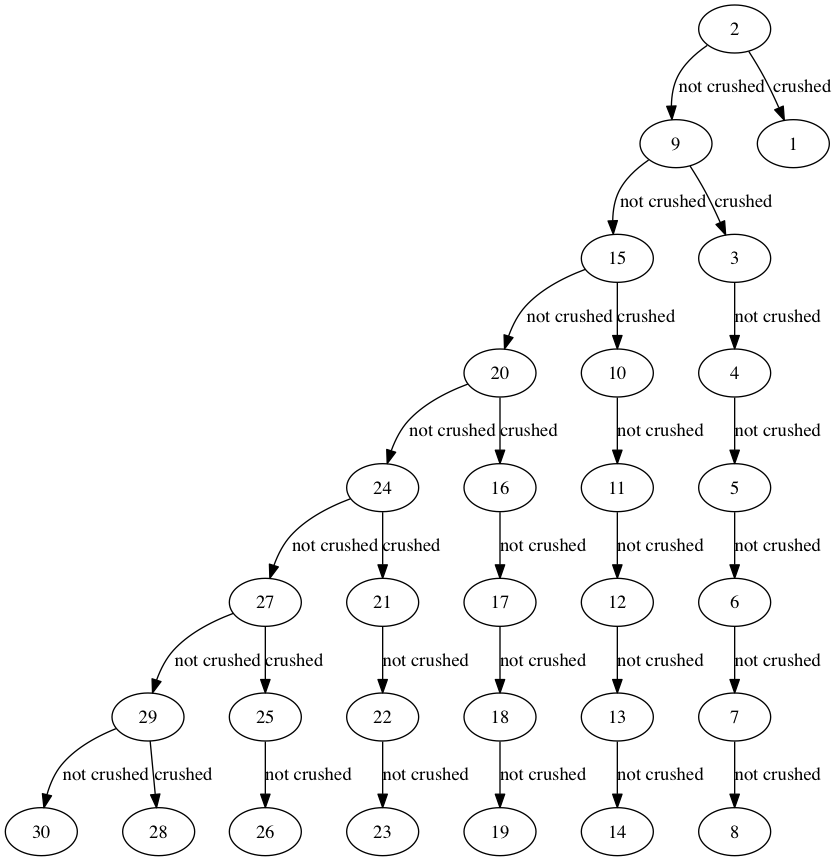
\includegraphics[width=\textwidth]{DecisionTree1}
		\caption{Optimal tree with smallest value of optimum level}
		\label{fig:badtree}
	\end{subfigure}
	\begin{subfigure}{0.68\textwidth}
		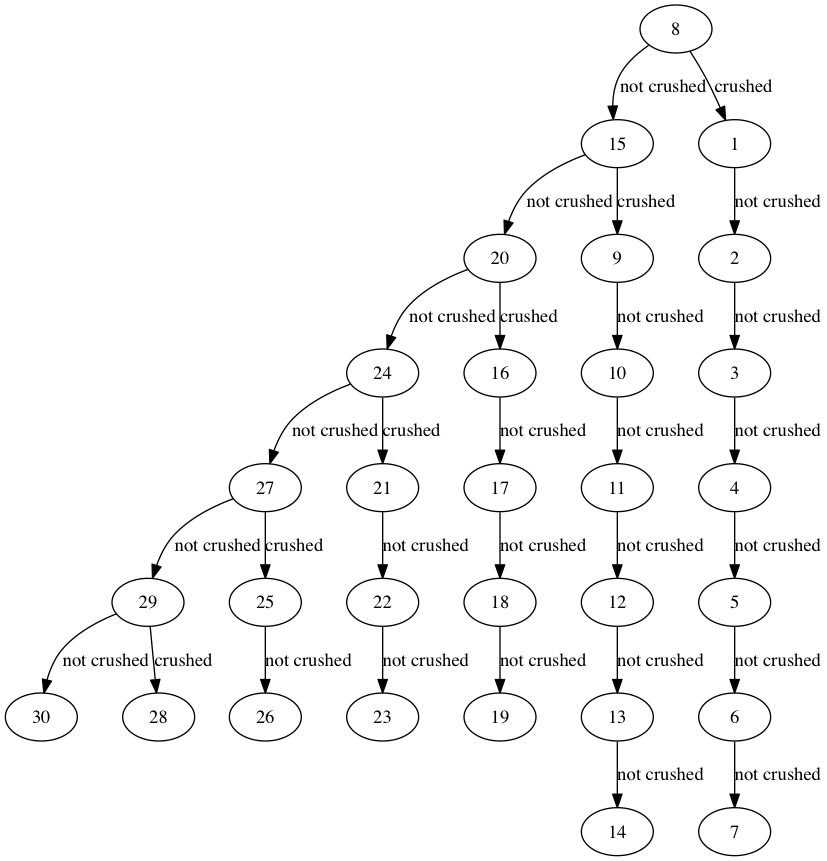
\includegraphics[width=\textwidth]{DecisionTree2}
		\caption{Optimal tree with largest value of optimum level}
		\label{fig:goodtree}
	\end{subfigure}
	\caption{Optimal decision trees for 2 iPads and 30 strength levels}
	\label{fig:decisiontrees}
\end{figure}

Furthermore, if the player specifies a strength of level 9 to use, the game logic will make the correct decision to crush the iPad, as it will mean that the player has 1 iPad and 8 more levels to test, which is a trivial state that requires 8 attempts to complete. This gives a total of 9 attempts, which is worse than the best strategy that uses 8 attempts.

Now that we know we must choose 8 as our optimum level, what happens when the player chooses to use a strength level of 8? Should the game logic decide to crush the iPad or not? Will it make a difference? If we look at tree (b), we can quickly realise that if we make the game logic such that it does not crush the iPad, the player can follow down the decision tree and pick levels {8, 15, 20, 24, 27, 29, 30} subsequently to solve the game. This results in a total of 7 attempts, even though there is a longer path in our decision tree that needs 8 attempts. Therefore, by making the game logic such that it crushes when the optimum level is chosen, we can ensure that the player will always require at least $height + 1$ number of attempts to solve the game, which in this case will be 8.

There is an exception, however, and it happens when the player has only 1 iPad left. With only 1 iPad left, the player has to use the minimum strength that he is unsure of up to that point of the game, and slowly increase 1 level by 1 level until he reaches the maximum strength level he is unsure of. Since the optimum level in this case is the minimum strength level, if we follow the conditions above and crush the iPad when the player chooses this minimum level, the game will end earlier than expected. The player will know that minimum level - 1 is the highest strength level he can use. In order to maximise the number of attempts needed for the player to determine the highest strength level, we must ensure that the game logic checks if there is only 1 iPad left, and in that event, decides not to crush the iPad when the player chooses the minimum strength level. If the player does not choose the minimum strength level, then the iPad will be crushed and the player would have lost the game since he is left with 0 iPad and has not solved the game.

\section{Implementation of approach}
After considering the viability of the approach, we went on to figure out how we would implement this approach. Since there was not a clear and direct link of how the optimum level of smaller problems can help to determine the optimum level of a bigger problem, further exploration was needed. 

After trying out some ways that included using the decision tree to fill a $N$ by $L$ table of optimum strength levels, we concluded that the more straightforward way is to simply keep both the cost (height of optimum tree) and the optimum level for each cell in the table. This would mean that the way we are implementing this approach is to extend upon our original solution, where instead of just storing the cost in each cell, we will also store the largest level that gives us this minimum cost. This will allow us to populate the table easily, by using the same way we did in Chapter 2.

\section{Advantages and disadvantages}
If the implementation of this approach is just an extension of our original solution, what are the advantages of storing the optimum level in each cell of our table? Are there any disadvantages as well? 

As mentioned by Prof. Sim, the advantage of knowing the optimum level of every game state will allow us to give the player hints of which strength level he should use. An example of a hint can be in the form of mathematical equations to be solved to indicate a range of values that includes the optimum level. This can provide a "side-game" for players and make the game more interesting, increasing the overall entertainment the game provides. 

There are some minor disadvantages though, and they include the conditions that were described earlier in this chapter. In order for the game logic to always output the worst case scenario for the player, we must take note of those conditions and be mindful when implementing the game logic.

%===============================================================================
% End of Chapter 4
%===============================================================================

%===============================================================================
% Start of Chapter 5
%===============================================================================
\chapter{The online combinatorics approach}
Besides the Dynamic Programming approach to this iPad Crushing problem, we also found an interesting alternative approach online using Combinatorics to calculate how many times we need to crush the iPad in the worst case \cite{randomblogpost}. The original author describes it as a solution to the classic Egg Dropping Puzzle. Here, we formulate the solution in terms of our iPad Crushing problem and make some corrections.

\section{Theory}
Before we begin discussing the solution, we need to reiterate our definition of a strategy to solve the iPad Crushing problem. A strategy is a binary decision tree, with each node representing a level of strength that we will use to try crushing the iPad. Following the left branch represents the scenario that the iPad survives the crush, while the right branch represents the scenario when the iPad does not survive the crush. A leaf of the tree represents the the minimum level of strength to crush the iPad that we have found.

The number of crushings we need to do to determine the minimum strength level to crush the iPad is the length of a path from the root node to a leaf. Hence, the number of crushings in the worst case is just the height of the decision tree. The goal of the game is to find a decision tree with minimum height.

Similar to the dynamic programming approach, given the number of levels $L$ and the number of iPads $N$, we will need to find the minimum height $H$ of a decision tree to solve this iPad Crushing Problem. However, we will do this by formulating a slightly different problem. This is quite similar to the proof that all comparison-based sorting algorithms need to make at least $\log n$ comparisons in the worst case. An iPad Crushing problem with $N$ iPads and $L$ strength levels has a decision tree of height $H$. We will find the maximum $L$, given $N$ and $H$.

We will count the number of possible paths in the decision tree of height $H$. The number of paths is equal to the number of  leaves, which is exactly $L+1$, as there are $L+1$ possible values for the minimum strength level to crush the iPad.

In addition, every path from the root node to a leaf can branch to the right (the iPad does not survive) at most $N$ times. Hence each path can be represented by a binary sequence of 1 (left) and 0 (right), with at most $N$ zeros (rights). Since the height of our decision tree is $H$, the length of each path is at most $H$. For a path with length less than $H$, we can append it with ones such that the length of its binary sequence representation is always $H$. This is a one-to-one transformation because no path's binary sequence can be contained in another. Hence we have a bijection between the set of possible paths and the set of binary sequence of length $H$ with at most $N$ zeros. There are ${H \choose k}$ binary sequences of length $H$ with $k$ zeros. Therefore, the maximum number of paths in a decision tree of height $H$ is $\sum_{k=0}^{N} {H \choose k}$.

Combine the previous two paragraphs, we arrive at the inequality: \[\sum_{k=0}^{N} {H \choose k} \geq L+1\]

So back to our original problem, the decision tree for this iPad Crushing problem with $N$ iPads and $L$ strength levels will have the minimum height $H$ such that the above inequality holds.

\section{Algorithm}
Based on the theory discussed in the previous section, together with the fact that $H \geq \log L$ since the decision tree is a binary tree, we formulate the following algorithm to calculate the cost in the worst case of the iPad Crushing problem.

\begin{algorithm}
        \caption{Calculate the cost of the iPad Crushing problem with N iPads, L strength levels}
        \begin{algorithmic}[1]
            \REQUIRE N, L
	\STATE $H \leftarrow \lceil \log L\rceil$
	\STATE $sum \leftarrow \sum_{k=0}^{N} {H \choose k}$
	\WHILE {$sum < L+1$}
		\STATE $H \leftarrow H+1$
		\STATE $sum \leftarrow \sum_{k=0}^{N} {H \choose k}$
	\ENDWHILE
	\RETURN $H$
        \end{algorithmic}
\end{algorithm}

\section{Discussion}
We can use the algorithm outlined in the previous section to fill in our $N \times L$ DP table. The running time of this algorithm is dependent on the size of the answer it gets, which grows slower than $O(L)$ - the cost to fill in one entry for the dynamic programming approach\footnote{This is our observation. We do not have enough mathematical knowledge to prove it.}. Hence, we would expect that this algorithm runs faster than the dynamic programming one. Our tests verify this hypothesis. Therefore, an advantage of this approach would be its faster running time.

However, the downside of this approach is that it is harder to tweak to solve modified versions of the iPad Crushing problem. We tried to tweak it to solve the problem when the cost of an iPad is 5. What we have come up with is, to replace each branch to the right with 6 consecutive branchings to the right. Hence the total number of possible paths will be the number of binary sequences of length $H$ such that zeros can only appear in group of 6, and there are at most $N$ groups of 6 zeros. To solve this, we need to consider a group of 6 zeros as one units (one 0), which decreases the length of the sequence to $H - 5 \times number\_of\_groups$. This gives us a more complicated inequality: \[\sum_{k=0}^{N} {H-5k \choose k} \geq L+1\]

We can also modify this approach to solve the problem when there are inifinitely many available iPad for use. Instead of summing until $N$, we can sum until ${H-5k \choose k}$ still makes sense, that is until $\lfloor H/5 \rfloor$. This gives us the inequality: \[\sum_{k=0}^{\lfloor H/5 \rfloor} {H-5k \choose k} \geq L+1\]

A modification can also be made to solve the problem with dynamic iPad cost. Let $f(x)$ be the function that return the cost of the $x^{th}$ iPad crushed. We define the function $S(x)$ as the sum of the cost of the 1st $x$ iPads crushed, i.e.: \[S(x) = \sum_{i=0}^x f(i)\] The core inequality essential to the combinatoric method will then become: \[\sum_{\substack{k \in \mathbb{Z}_{\geq 0}\\ S(k) < H}} {H-S(k) \choose k} \geq L+1\]

%===============================================================================
% End of Chapter 5
%===============================================================================

%===============================================================================
% Start of Chapter 6
%===============================================================================
\chapter{Interesting extensions}
\section{iPad with fixed cost}

What happens if we have to pay a penalty for each crushed iPad. How would it affect the game logic?

To tackle this extension, we realise we can re-use our cost table approach, but modify the comparison step slightly to also include the fixed cost. 

Using the table cost approach, we would calculate the cost of the whole DP table during the game initialisation, and subsequently use the value already calculated in the table cell to make the game decisions

In this extension, we consider two scenarios: The number of iPads is finite or infinite

\subsection{Finite number of iPads}

In the case that there is a finite number of iPads, the DP table will be a 2D array, where the number of rows represent the number of iPads, and the number of columns represents the number of levels

The pseudo code to calculate the DP table is as follows

\begin{algorithm}[H]
\caption{Calculate the cost table for fixed iPad cost (finite number of iPads}
\begin{algorithmic}[1]
\REQUIRE N, L, iPadCost
\STATE $table \leftarrow 2DTable(N, L)$
\FOR{$i = 0$ \TO $N$}
	\FOR{$j = 0$ \TO $L$}
		\STATE $table[i][j] = \infty$
	\ENDFOR
\ENDFOR
\FOR{$i = 0$ \TO $N$}
	\FOR{$j = 0$ \TO $1$}
		\STATE $table[i][j] = j*(1 + iPadCost)$
	\ENDFOR
\ENDFOR
\FOR{$i = 1$ \TO $L$}
	\STATE $table[1][i] = i + iPadCost$
\ENDFOR
\FOR{$i = 1$ \TO $N$}
	\FOR{$j = 1$ \TO $L$}
		\STATE $best \leftarrow \infty$
		\FOR{$k = 1$ \TO $j$}
			\STATE $result = max(table[i - 1][k - 1] + iPadCost, table[i][j - k])$
			\IF{$result < best$}
				\STATE $best \leftarrow result$
			\ENDIF
		\ENDFOR
		\STATE $table[i][j] = best + 1$
	\ENDFOR
\ENDFOR
\end{algorithmic}
\end{algorithm}

We can see that the difference between this and the previous cost table approach without iPad cost is only that the iPad cost is also added to the original cost in each cell

\subsection{Infinite Number of iPads}

In the case that there is an infinite number of iPads, the DP table only needs to be a 1D array. Since the number of iPads is infinite, we no longer need to worry that we might run out of iPads. As such, we only need to consider how the cost will vary by the level. The number of cells in the DP table (or in this case the DP row) hence represents the number of levels

The pseudo code to calculate the DP table is as follows

\begin{algorithm}[H]
\caption{Calculate the cost table for fixed iPad cost (infinite number of iPads)}
\begin{algorithmic}[1]
\REQUIRE L, iPadCost
\STATE $table \leftarrow 1DTable(L)$
\FOR{$i = 0$ \TO $L$}
	\STATE $table[i] = \infty$
\ENDFOR
\STATE $table[0] = 0$
\STATE $table[1] = iPadCost$
\FOR{$i = 2$ \TO $L$}
	\STATE $best \leftarrow \infty$
	\FOR{$k = 1$ \TO $j$}
		\STATE $result = max(table[k - 1] + iPadCost, table[j - k])$
		\IF{$result < best$}
			\STATE $best \leftarrow result$
		\ENDIF
	\ENDFOR
	\STATE $table[i] = best + 1$
\ENDFOR
\end{algorithmic}
\end{algorithm}

\section{iPad with dynamic cost}
Let's make the problem even more complex. How do we tackle the problem if the cost of the iPad is not fixed, but changing depending on how many iPad has been crushed. 
We can first define a function f, where f(n) denotes the cost of the $n^{th}$ being dropped.
Intuitively, we can see that this problem is very close to the fixed iPad cost problem. We can again use the cost table. approach to pre-calculate the DP cost table. The difference lies in the fact that we also now need to consider how many iPads have been crushed before.
Therefore, to extend the solution for the fixed cost problem to also work in this, we can also store an attribute denoting the number of Ipad crushed. Each cell will then have two attributes, the cost and the number of iPad crushed
The pseudo code to calculate the DP table is as follows

\begin{algorithm}[H]
\caption{Calculate the cost table for dynamic iPad cost}
\begin{algorithmic}[1]
\REQUIRE N, L, f
\STATE $table \leftarrow 2DTable(N, L)$
\FOR{$i = 0$ \TO $N$}
	\FOR{$j = 0$ \TO $L$}
		\STATE $table[i][j].cost = \infty$
		\STATE $table[i][j].numberOfiPadCrushed = 0$
	\ENDFOR
\ENDFOR
\FOR{$i = 0$ \TO $N$}
	\FOR{$j = 0$ \TO $1$}
		\STATE $table[i][j].cost = j*(1 + f(j))$
		\STATE $table[i][j].numberOfiPadCrushed = j$
	\ENDFOR
\ENDFOR
\FOR{$i = 1$ \TO $L$}
	\STATE $table[1][i].cost = i + f(1)$
	\STATE $table[1][i].numberOfiPadCrushed = 1$
\ENDFOR
\FOR{$i = 1$ \TO $N$}
	\FOR{$j = 1$ \TO $L$}
		\STATE $best \leftarrow \infty$
		\FOR{$k = 1$ \TO $j$}
			\STATE $ipadCostWhenCrushed =  f(table[k-1][i-1].numberOfiPadCrushed +1)$
			\STATE $result = max(table[i - 1][k - 1] + iPadCost, table[i][j - k])$
			\IF{$table[j-k][i].cost >= table[k-1][i-1].cost + ipadCostWhenCrushed$}
				\STATE $resultCost= table[j-k][i].cost$
				\STATE resultNumberOfiPadCrushed $= table[j-k][i].numberOfiPadCrushed$
			\ELSE
				\STATE $resultCost= table[k-1][i-1].cost + ipadCostWhenCrushed$
				\STATE $resultNumberOfiPadCrushed = table[k-1][i-1].$numberOfiPadCrushed $+ 1$	
			\ENDIF
			\IF{$resultCost < best$}
				\STATE $best \leftarrow resultCost$
			\ENDIF
		\ENDFOR
		\STATE $table[i][j].cost = best + 1$
	\ENDFOR
\ENDFOR
\end{algorithmic}
\end{algorithm}

%===============================================================================
% End of Chapter 6
%===============================================================================

%===============================================================================
% Start of Chapter 7
%===============================================================================
\chapter{Conclusion}
Lorem ipsum dolor sit amet, consectetur adipiscing elit. Duis quis lacus posuere, tincidunt mauris vitae, bibendum sapien. Suspendisse a eros pretium, pretium libero eget, ornare ante. Donec efficitur gravida pellentesque. Curabitur sit amet pulvinar tortor. In eu risus commodo, elementum tellus ac, commodo mauris. Vestibulum ante ipsum primis in faucibus orci luctus et ultrices posuere cubilia Curae; Integer hendrerit arcu sem, convallis dignissim nisi faucibus at. Praesent ut rutrum libero, sollicitudin blandit dui. Donec mi nisi, cursus quis accumsan et, molestie ut nisi. Sed egestas enim in dolor tincidunt dictum. Sed eu semper sem. Sed elementum augue ac pretium eleifend. Ut massa tortor, rhoncus a mi ac, congue ullamcorper eros. Maecenas imperdiet orci quis dui rhoncus, id rhoncus mi condimentum. Nunc blandit egestas leo, sit amet porttitor mi malesuada nec. Pellentesque id bibendum purus, a porta risus.

%===============================================================================
% End of Chapter 7
%===============================================================================

%===============================================================================
% Start of References
%===============================================================================
\renewcommand{\bibname}{References}
\begin{thebibliography}{1} \addcontentsline{toc}{chapter}{References}
	\bibitem{randomblogpost} Egg Drop Puzzle. http://michaelbrundage.com/note/2014/04/26/egg-drop/
\end{thebibliography}

%===============================================================================
% End of References
%===============================================================================
\end{document}
